%%%%%%%%%%%%%%%%%%%%%%%%%%%%%%%%%%%%%%%%%%%%%%%%%%%%%%%%%%%%%%%%%%%%%%%%
%    INSTITUTE OF PHYSICS PUBLISHING                                   %
%                                                                      %
%   `Preparing an article for publication in an Institute of Physics   %
%    Publishing journal using LaTeX'                                   %
%                                                                      %
%    LaTeX source code `ioplau2e.tex' used to generate `author         %
%    guidelines', the documentation explaining and demonstrating use   %
%    of the Institute of Physics Publishing LaTeX preprint files       %
%    `iopart.cls, iopart12.clo and iopart10.clo'.                      %
%                                                                      %
%    `ioplau2e.tex' itself uses LaTeX with `iopart.cls'                %
%                                                                      %
%%%%%%%%%%%%%%%%%%%%%%%%%%%%%%%%%%
%
%
% First we have a character check
%
% ! exclamation mark    " double quote  
% # hash                ` opening quote (grave)
% & ampersand           ' closing quote (acute)
% $ dollar              % percent       
% ( open parenthesis    ) close paren.  
% - hyphen              = equals sign
% | vertical bar        ~ tilde         
% @ at sign             _ underscore
% { open curly brace    } close curly   
% [ open square         ] close square bracket
% + plus sign           ; semi-colon    
% * asterisk            : colon
% < open angle bracket  > close angle   
% , comma               . full stop
% ? question mark       / forward slash 
% \ backslash           ^ circumflex
%
% ABCDEFGHIJKLMNOPQRSTUVWXYZ 
% abcdefghijklmnopqrstuvwxyz 
% 1234567890
%
%%%%%%%%%%%%%%%%%%%%%%%%%%%%%%%%%%%%%%%%%%%%%%%%%%%%%%%%%%%%%%%%%%%
%
\documentclass[12pt]{iopart}
\usepackage{graphicx}
\usepackage[sf]{subfigure}
\newcommand{\gguide}{{\it Preparing graphics for IOP journals}}
%Uncomment next line if AMS fonts required
%\usepackage{iopams}  

\begin{document}
\bibliographystyle{unsrt}

\title[Macro drop and droplet profile detection during PGMAW process by image processing]{Macro drop and droplet profile detection during PGMAW process by image processing}

\author{E Romero, C Bordreuil, J Chapuis, F Souli\'e, G Fras}

\address{Laboratoire de M�canique et G�nie Civil,
CC048, Place Eug�ne Bataillon, Universit� Montpellier 2,
34095 Montpellier, France}
\ead{cyril.bordreuil@univ-montp2.fr}

\begin{abstract}

\end{abstract}

%Uncomment for PACS numbers title message
%\pacs{00.00, 20.00, 42.10}
% Keywords required only for MST, PB, PMB, PM, JOA, JOB? 
%\vspace{2pc}
%\noindent{\it Keywords}: Article preparation, IOP journals
% Uncomment for Submitted to journal title message
%\submitto{\JPA}
% Comment out if separate title page not required
\maketitle

\section{Introduction}

A better comprehension of  behavior of the weld pool or the metal droplet  in a PGMAW process
 could help to improve numerical simulations
 and enhance welding quality in manufacturing process \cite{LIN}, \cite{WU1}.
% An example to this are the problems linked to productivity. To some process,
 For example, the
 increase of productivity means often increase of welding speed.
 However welding defects  related to bad shape, as the hump formations, limit the maximum weld 
 speed \cite{CHAPUIS,Mendez} and therefore the productivity. 
 In a PGMAW process, the weld quality is strongly relates with the metal transfer  stability 
 (the droplet deposition). The control of metal transfer process %implies control of
 will improve weld quality \cite{WANG}. In both example cases a macro drop kinetic
  study and a droplet dynamic analysis during static PGMAW process could help to better
 understand some GMAW related phenomena as humping formation \cite{CHO}, droplet 
  fluctuations \cite{WANG} that guarantee the welding quality. 
 In both case, the kinetic and the dynamic analysis, required the monitoring \cite{} and the 
  geometrical analysis of macro drop and droplets in order to extract 
  qualitative information of these welding entities. 

There have been many studies on visual sensing techniques for observing weld pool 
image \cite{BAE} and metal transfer process during welding \cite{LIN}.
Optical sensors like high speed  cameras and lighting systems have been
widely use in GMAW process to realize  image acquisition \cite{ZHANG4},
control process \cite{BAE}, parametric studies \cite{BALSAMO} and droplet dynamics analysis\cite{LIN}.
Image processing plays a critical role in extracting useful information from visual scenes \cite{WANG}.
Nevertheless the strong interference from the arc lightning required more than standard 
image treatment to analyses the raw images of the welding process \cite{NORDBRUCH}. 
Previous work has shown that is possible to perform geometrical 
analysis in weld pools or droplets \cite{WU1}.
Parameters such as macro drop or droplets surface, volumes 
or height has been measure using different and 
specific processing images algorithms \cite{WANG}, \cite{WU1}, \cite{SEED},
\cite{NORDBRUCH}. However, to date, effectively automatic images processing
of metal transfer has not been developed, possibly due to the  difficulty involved 
for welding researchers \cite{WANG}. 

To perform geometrical analysis in macro drope and droplet;
 a multipurpose C++ based library (erCv) was developed at the lab. 
These library results from selected functions  from highly reliable 
open source libraries to images treatment, geometrical 
analysis, graph theory applications and image visualization.
In a first step, and despite the different static and dynamic weld conditions, 
as well as different current regime. A reliable 2D profiles and geometrical
parameters from macro drop and droplets, has been obtained using the mentioned library.
 Using this, a dimension and dimensionless analysis will 
be done. The intention is to help to simplified futures numerical models of humping phenomena and quality process.
     
The paper is organized as follows. First, the purpose of the library is explained, then 
the experimental setup that will allow to appreciate the performance of the algorithm,
 to study macro drop analysis is detailed. The library and the algorithms
developed are explained and some results are shown on the macro drop and droplet study.



\section{Problems description}

Bradstreet was the first researcher to experimentally study the bead hump formation \cite{CHO}. 
Humping was defined as the series of undulations of the weld bead. Further studies as computer 
simulation made by CHO et al. \cite{CHO} shown a relation between the droplet momentum deposition
 and the hump size. Same relations has been found between metal transfer process and welding quality \cite{}
% Il semble alors important de quantifier exp�rimentalement des donn�es

Then the shape and kinetic analysis of macro drop and droplets could help to better understand 
and enhance the PGMAW process. To monitoring the shape and size of these welding objects, to a 
first step, a 2D approach would be sufficient. Therefore a shadowgraphy technique, or back lighting,
is the natural choice to record the droplets and macro drops profiles \cite{BALSAMO}, furthermore is 
one of the only way to access these quantities. Due to the arc light interference and the relatively high 
speed of wire feed process, a high speed camera and an effective image processing algorithms are 
required \cite{WANG}. The typically frame rate acquisition to metal transfer drop kinetic analysis is $3000$ 
per second \cite{WANG}. Therefore the algorithms have to be able to extract 
the geometrical information (area, size and others) from the macro drop and droplets,
from a huge amount of data. In addition, the voltage and current signals are directly related 
with the droplet formation at the wire \cite{BALSAMO}.
% Good synchronizations methods have to 
%be applied between shadowgraphies 
%frames and electrical signals.



\section{Image processing background} 

Some definitions and brief description of generals principles used in
 image processing are required to better understand  the 
algorithms and the design of the library.

\subsection{Some definitions}\label{some_definitions}
A numerical grey image can be describe as 3D surface discretized by a grid mesh
 in the X,Y plane. Each mesh represents a pixel and the relief surface at Z axis,
 the grey level. 
A strong relief change or high gradient greyness values at
 the image are perceive by human eyes as light changes, and can be interpreted
 as objects edges. 

Sometimes, a regular relief patrons or regular greyness
 variation can be distinguish. The human eyes can perceive these patrons as texture 
and interpret the space between different textures zones as edges.
There exist a large spectrum of algorithms to image treatment, in particular to edges detect.
 Most of them can be classified by the way that his operate above the image pixels and grey level.

\subsection{Filters}\label{filters}

The filters are algorithms that operate as mathematical functions $f$ above the 
$X$, $Y$ or both axis of the image ($Z = f(X,Y)$,  
$f(X)$ or $f(Y)$)  modifying his greyness value or $Z$ component. 
Different kind of filters can be mentioned as median, Gaussian, impulse,
 adaptive and others. The impulse filters such Canny are 
widely use to edge detection \cite{COCQUEREZ}. These filter have an
 impulse response to most important greyness gradient in the 
image; this allows the filter a better edges localisation
 (see figure \ref{photo-explication-filter}). 
For this reason, Canny filter is widely 
used in the library to detect the welding elements edges. 
However, it is sensible to noise or secondary greyness gradients in the image
 and, in consequence, it have some difficulties to define closer surface.

\subsection{Snake and level set}
\label{snake-and-level-set}
 
Curve propagation is a popular technique in image analysis for object extraction,
 object tracking, edge detection and others (see figure 
\ref{photo-explication-snake}). The central idea behind such an approach
 is to evolve a curve towards the lowest potential of a cost function. 
However at each stage of curve evolution, each curve point potential has
 to be computed. A lot of point (better curve resolution) take a lot 
computing time, and therefore are not yet apply to real time detection
 or relatively speed automatic image processing. For this reason snake algorithms are not used in the library.

\subsection{Segmentation}
\label{segmentation}

Let $B$ an image and let $R_{i}$ a region of $B$ such:

\begin{eqnarray}
B = \bigcup_{i}R_{i}\ \forall i \in \{0, \mbox{numbers of regions in B}\} \\
\mbox{with} R_{i} \neq \emptyset \\
\mbox{and}  R_{i}\bigcap R_{j} = \emptyset  \forall i, j\ \mbox{with}\ i \neq j\ 
\label{equation-segmentation}
\end{eqnarray}

A $B$ segmentation is an image treatment which generate a $B$ partition in $R_{i}$ regions. 
Each region is a connected set of pixels with 
common properties (intensity, texture,...) \cite{COCQUEREZ}.
 The partition is generated by operations or comparisons methods between 
regions. Generally, this treatment offers a good detection edges if
 the elements and surrounding area have different textures (see figure
 \ref{photo-explication-segmentation}). 
Note that different regions can belong to the same partition and not
 be placed together, therefore the surface is not always connected and,
 in consequence, the edges of the interest regions are not always closed.

\begin{figure}[h!]
\begin{center}    
\subfigure[Weld pool image in static GTAW process]{\label{photo-explication-patron}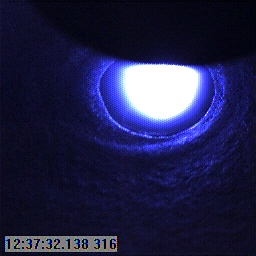
\includegraphics[width=3.5cm,height=3.5cm]{images/photo-explication-patron.png}}
\subfigure[Canny filter treatment]{\label{photo-explication-filter}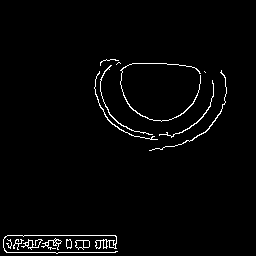
\includegraphics[width=3.5cm,height=3.5cm]{images/photo-explication-filter.png}}\\
\subfigure[Snake treatment]{\label{photo-explication-snake}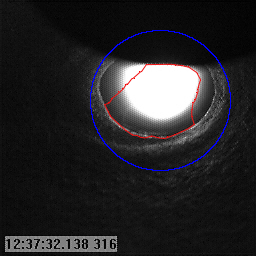
\includegraphics[width=3.5cm,height=3.5cm]{images/photo-explication-snake.png}}
\subfigure[Segmentation image by 2 cluster sample comparison]{\label{photo-explication-segmentation}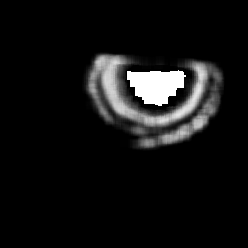
\includegraphics[width=3.5cm,height=3.5cm]{images/photo-explication-segmentation.png}}
\end{center}
\caption{{\small Samples of different methods technique for image processing}}
\label{photo-explication}
\end{figure}


\section{Image treatment library (erCv)}
\label{image-treatment-library-ercv}

As mentioned, a multipurpose image processing library was developed 
and currently use at the laboratory, in order to analyze welding process objects.
erCv is able to perform edge detection and geometrical analysis in a different 
welding objects such: Macro drop, droplets and weld pool.
erCv is a modular library assembled in a oriented object C++ language. Then erCv is a scalable 
and portable library able to perform real time
 contour detection. erCv is implemented in  C++ with some bindings in python,
 making it relatively convivial to use.
erCv is compose by four processing modules based in C,  C++ and python language (see figure \ref{schema-erCv}). These modules are: 
\begin{description}
\item[Image Treatment:] Due to weld process conditions such arc lightening, 
 heat and electrodes positions; the raw image registered by CCD 
 camera are not calibrated and present light inhomogeneities and 
 noise. In order to obtain the real shape and size of weld elements, this module 
 include calibrations algorithms. To detect the welding objects contours it is 
 necessary to improve the weld element image. This module has the 
 pre-processing treatments to noise reduction and image enhancement.
 Then to start the edges detection process, this module includes processing
 algorithms as segmentations by samples comparators, watershed transformation,
 filters edge detectors and histogram based methods.  
\item[Geometrical Treatment and Analysis:] This module convert edges pixels points into connected 
   segments to end the edge detection
  process, completing and in some cases extrapolating the weld
  elements edge. It is also responsible to compute the geometrical 
  data of welding elements such weld pool surface and metal transfer drop volumes. 
  This module uses a full geometry algorithm library\cite{CGAL}, which include different algorithms
  such as triangulations and mesh generation, alpha shape and 
  convex hull generation and polygonal structures.
\item[Graph Theories:] To compute the geometrical data of welding elements
   it is necessary to extract the welding object edge from the image; this
   required some criteria such as continuity, length or closer condition.
   This module use graph algorithms to  identify and select the welding element edge using the
   criteria. This module is composed by connected segments, estimates
   minimal cut, determine largest chain segments and others algorithms. 
\item[Visualization:] This module is a set of 
  functions use to execute, show and/or register the 
  different steps at the image process.
\end{description}

\begin{figure}
\begin{center}
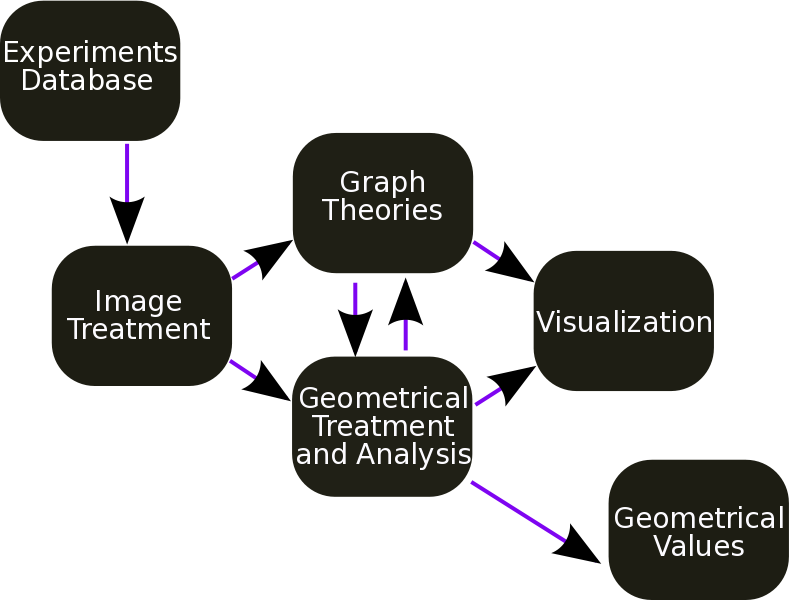
\includegraphics[width=7cm,height=4cm]{images/schema-erCv.png}
\caption{{\small Flow diagram of erCv library composition}}
\label{schema-erCv}
\end{center}
\end{figure}


\section{Experimental Setup}
\label{experimental_setup}

\subsection{Multi-physics platform}
\label{multi_physics_platform}

The objective is to perform geometrical analysis and measure characteristic
times of the macro drop and the droplet in a PGMAW process. Notes that
geometrical analysis refers to area section of droplets, height profile
of macro drop and wetting contacts angles of the macro drop. 
And characteristic times measures refer to time to height stagnation 
of macro drop and fall time of droplet between electrodes. The method
is the image treatment 
of recorded image of PGMAW static process by a high speed CCD camera.
% cb : Je vois pas ce que ca fout la?
%--To perform the geometrical analyses, different signals have to be synchronizes and recorder \cite{CHAPUIS}; 
%--therefore an accurate, reliable and synchronizes  systems are requires due to the high amount
%-- of data and highly noisy environment (electromagnetic noise and arc light radiation). 

%--A platform has been developed at the laboratory to perform multi-physics measures 
%--in arc welding process (see figure \ref{schema-platform}). The platform 
%-- was conceive with an automatically procedure to synchronize, to acquire,
%-- to manage and to exploit large flow of multi-physical experimental data (up to 2 Go
%--  per test). This characteristic allows synchronizing (in time) the current and voltage signals with the acquired images.

%--\begin{figure}
%--\begin{center}
%--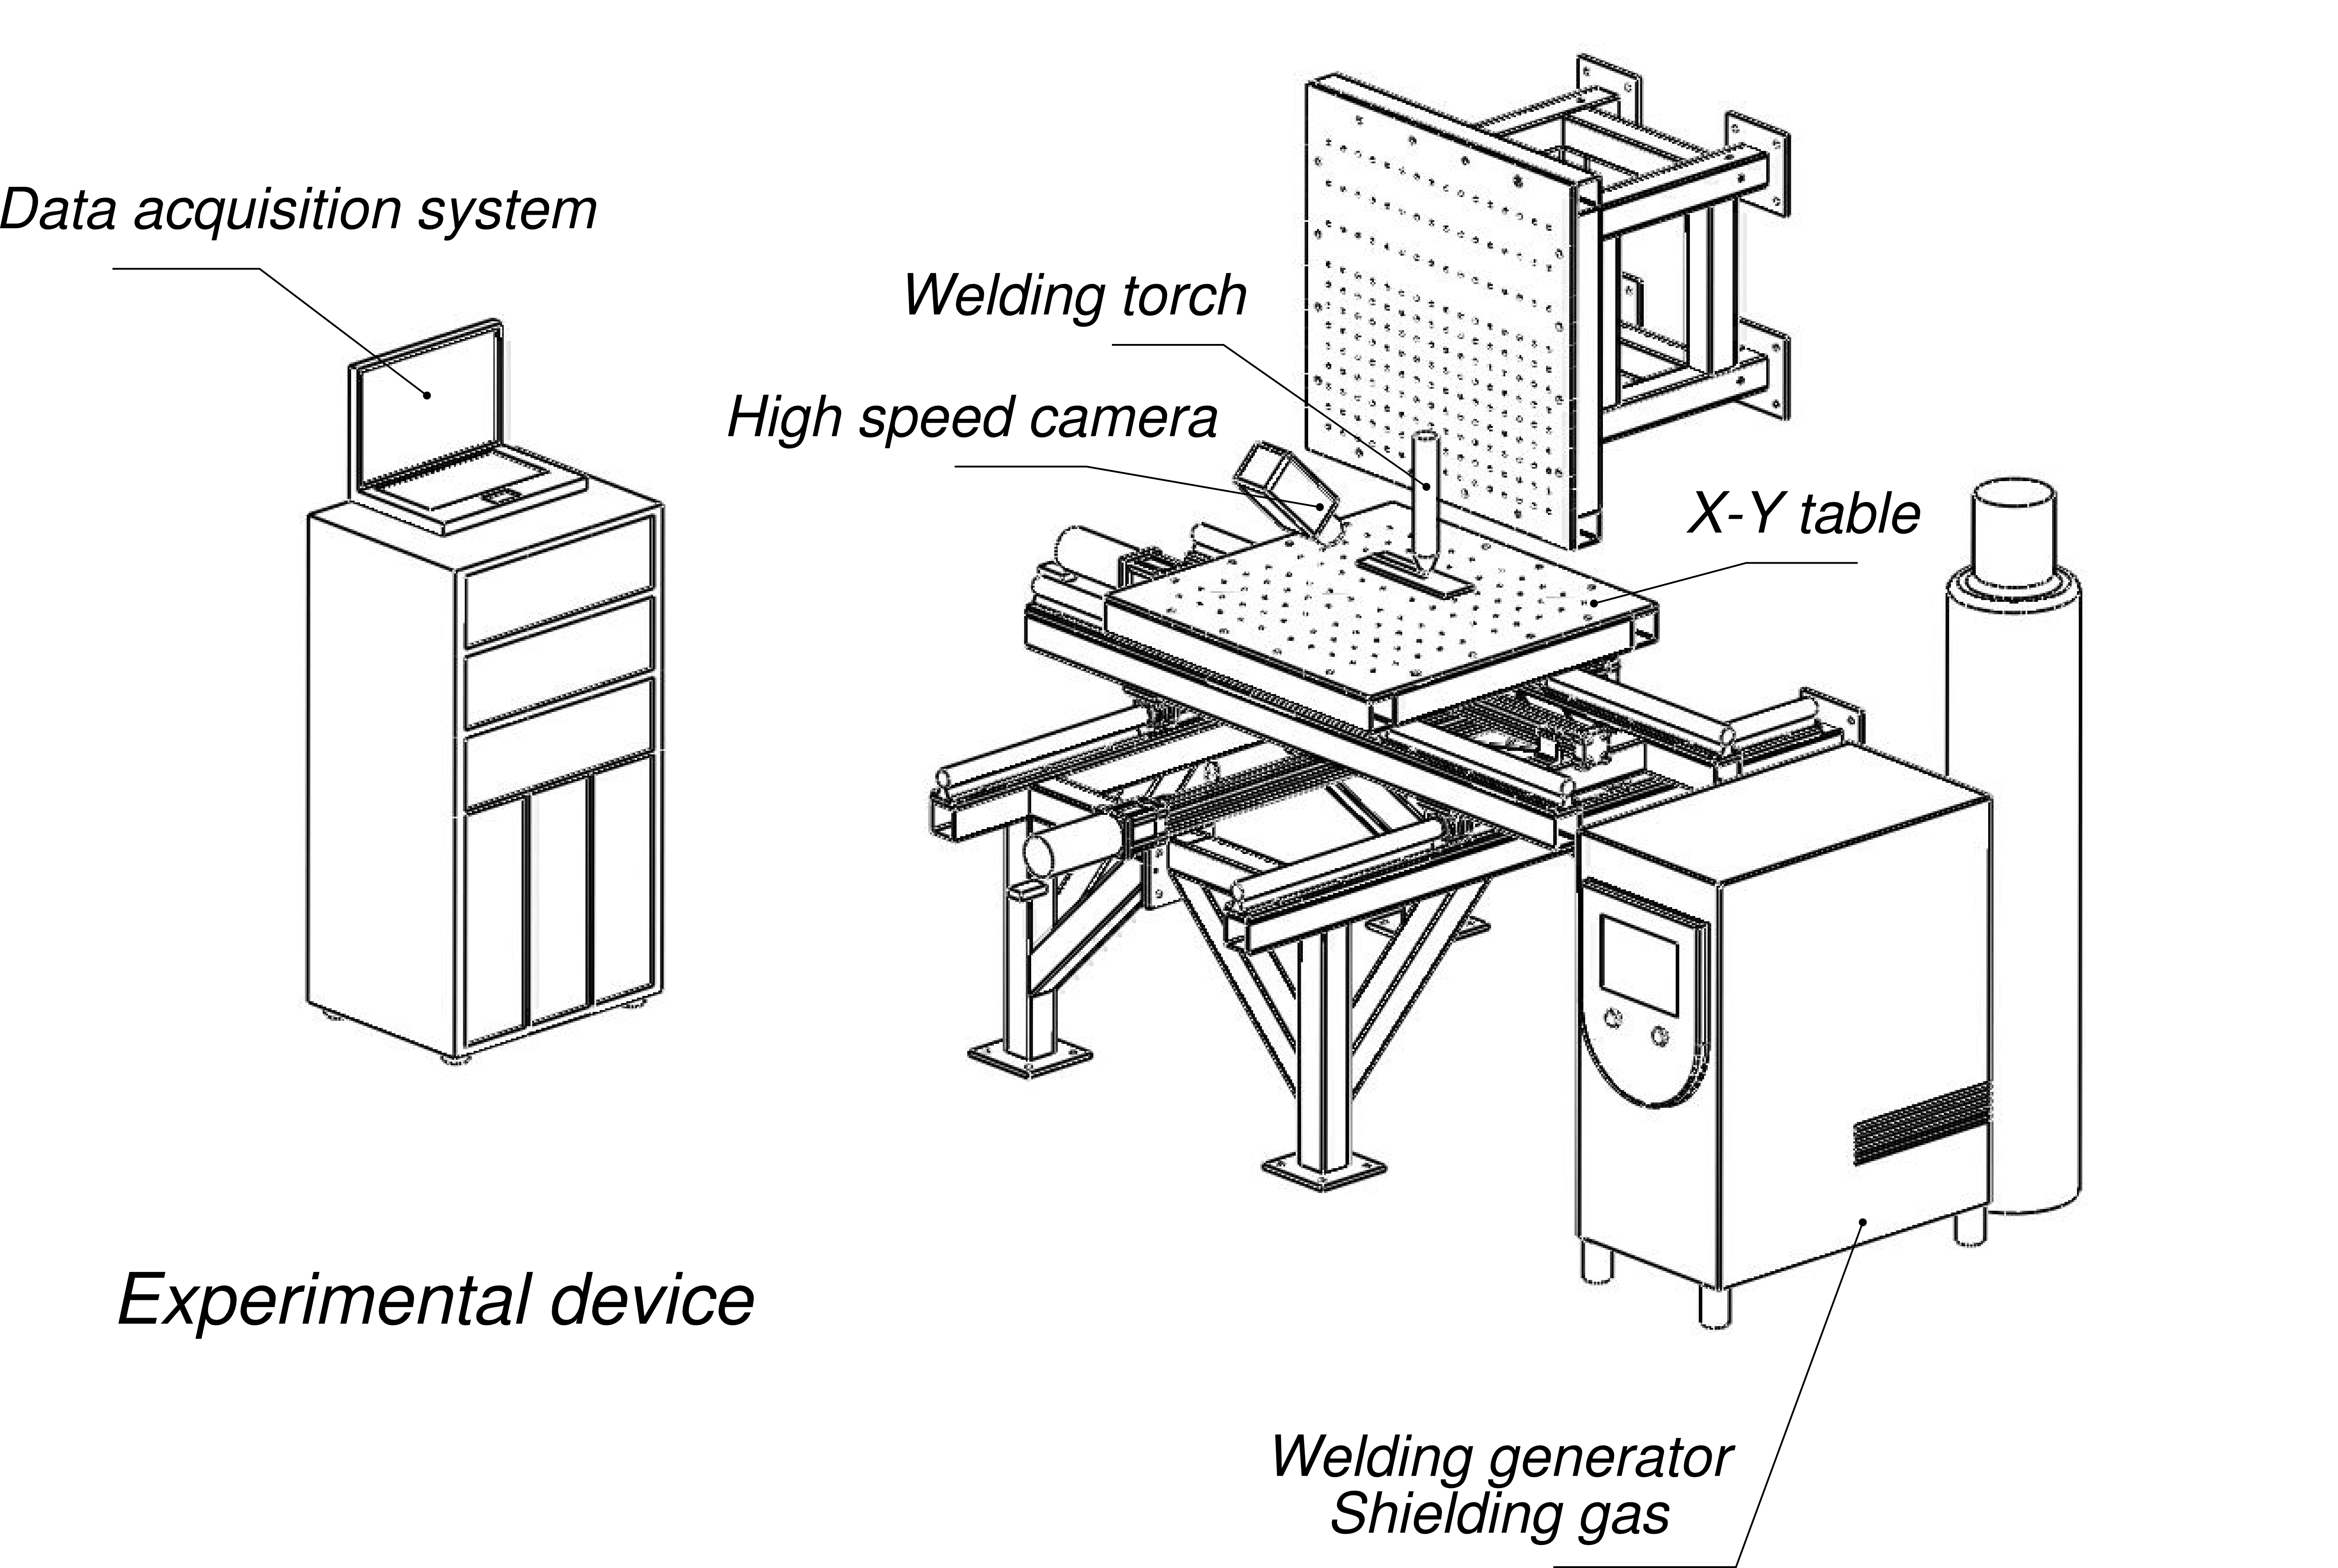
\includegraphics[width=7cm,height=4cm]{schema-platform.png}
%--\caption{{\small Experimental platform and specific device}}
%--\label{schema-platform}
%--\end{center}
%--\end{figure}

%--To compare and analyze the data two open source numerical libraries have been developed: The BAME (multi-physics measures data base) for all general data 
%--  and the erCv specific to image treatment (including the spreading of welding pool geometry during welding).



\subsection{ Image acquisition setup}
\label{ image_acquisition_setup}

The PGMAW static process is recorded by Shadowgraphy optical method. 
A halogen lamp is use to light the weld process. To guarantee a homogeneous
illumination of the welding process, a light diffuser is placed
in the optical path closer to the halogen lamp. 
Finally the shadows of welding elements are projected to the other side 
of the welding place. A Phantom V5.0 high speed camera is place and align 
at this side above the optical path (see figure \ref{schema-montage-experimental-GMAW}). 

\begin{figure}
\begin{center}
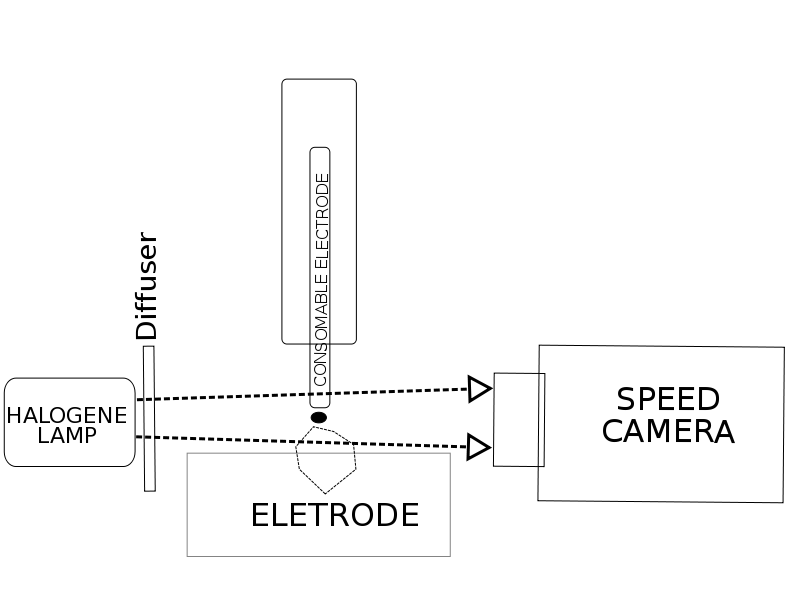
\includegraphics[width=7cm,height=4cm]{images/schema-montage-experimental-GMAW.png}
\caption{{\small Experimental setup to detect macro drop and droplet edges in GMAW process}}
\label{schema-montage-experimental-GMAW}
\end{center}
\end{figure}

To enhance the image contrast of the weld elements inside the electric discharge,
the intensity rate between arc light and halogen lamp have to be reduce. In order to this
a $650\ \pm 10\ nm$ band pass filter is place in front the camera lens, 
to attenuate the arc light. Nevertheless, the raw images remain highly 
noisy by the arc light. 


\subsection{ Welding condition}
\label{ welding_conditions}

Stationary spots weld are made using the GMAW process with the Oerlikon CitoWave 500 generator. 
The target is a steel disk of $10\ mm$ of thickness and 
ER70S steel welding wire.
The test campaign began by a reference test, with parameters fixed to:  welding time $4\ s$,
 wire feed speed $6\ m/min$, frequency droplets $113\ Hz$ and 
percentage of shielding gas ($CO_{2}$) $8$ (so $92\%$ argon). 
Welding parameters values are summarized in tables \ref{table-parameters-static} to static and 
\ref{table-parameters-change} to variables parameters.

\begin{table}
\begin{center}
\begin{tabular}{|cc|}
\hline
Welding wire type & ER70S \\ 
Wire diameter ($mm$) or $drw$ & 1 \\  
Contact tip to work distance ($mm$) & 20 \\
Shielding gaz flowrate ($l/min$) & 18 \\ \hline
\end{tabular}
\caption{{\small Determined constant welding parameters used in experiments}}
\label{table-parameters-static}
\end{center}
\end{table}

\begin{table}
\begin{center}
\begin{tabular}{|cc|}
\hline
Welding wire type & ER70S \\ 
Wire diameter ($mm$) or $drw$ & 1 \\  
Contact tip to work distance ($mm$) & 20 \\
Shielding gaz flowrate ($l/min$) & 18 \\ \hline
\end{tabular}
\caption{{\small Variable welding parameters used in experiments}}
\label{table-parameters-change}
\end{center}
\end{table}


%Welding current and arc voltage are recorded at $30\ kHz$ sampling rate.
The images are recorded at $4000$ frames per seconds, which is enough to
measure macro drop radius and apparent liquid-solid contact angle histories. 
%The images and electrical signals are synchronize, thanks to the
%automatically approach made in the multi physics platform.

Measurements are made using the erCv library.
      
      
      
      
\section{ System definitions}
\label{system_definitions}
\subsection{ Macro Drop}
\label{ macro_drop}

The purpose is to study the evolution of weld pool object in
a GMAW process or macro drop. Therefore it is necessary to study the shape and spreading
of the macro drop according depositing droplets of feed wire. 

At figure \ref{schema-macro-drop-droplet-parameters} appears the geometrical 
elements to be study at the macro drop: the macro drop radius at the base $R_{m}$, 
the macro drop center height $h_{m}$, the macro drop volume $V_{m}$, the
penetration below the surface level $p$ and the wetting angles:
$\Theta_{m(al)}$, $\Theta_{m(ar)}$ (apparent) and $\Theta_{m(rl)}$, $\Theta_{m(rr)}$ (real).
With the indices $l$ and $r$ refer to left and
right angles. The indices: $m$ refer to macro drop, $g$ refer to gaz, $l$ refer
to liquid, $s$ refer to solid$/$substrate and $a$ refer to the droplet.

\begin{figure}
\begin{center}
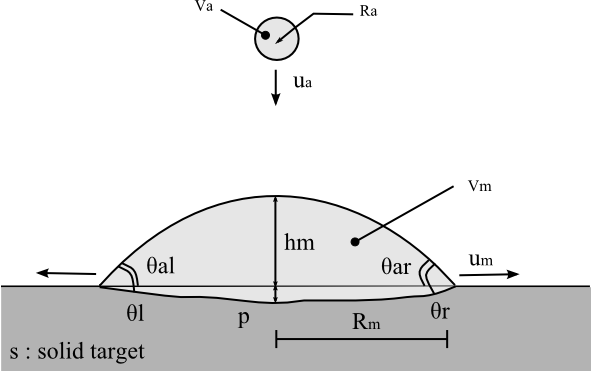
\includegraphics[width=7cm,height=4cm]{images/schema-macro-drop-droplet-parameters.png}
\caption{{\small Profile schematics of welding objects in a GMAW process}}
\label{schema-macro-drop-droplet-parameters}
\end{center}
\end{figure}
    
\subsection{ Metal Transfer Drop}
\label{ metam_transfer_drop}

To the droplet or metal transfer drop the geometrical parameters to identify are:
The estimate volume $V_{a}$ and the estimate radius $R_{a}$. 
Finally in order to better understand the droplet dynamic \cite{}, 
the physical elements to identify are: the fall time $t_{a}$ and the average 
speed $U_{a}$ (see figure \ref{schema-macro-drop-droplet-parameters}).



\section{ The Analyze methods}
\label{ the-analyze-methods}
\subsection{ Image Calibration}

As was shown in section \ref{image-acquisition-setup}, the camera recording a 
shadow projection of the welding process. The projection is 
supposed to be a section of the welding process image, orthogonal to the optical path.
Therefore, to a first approach, not image projection 
correction is necessary. Only to calibrate the image dimension 
(at pixels) to the real objects dimension (at millimeters), a conversion scale is 
made with the known width of the welding wire $conv = 1\ mm/ 20\ pixels$ . 
  
  
\subsection{ Image Treatment}
\label{ image_treatment}

The idea is to extract the macro drop and droplet shapes 
from the raw images and therefore to extract the geometrical information.
 The most common approach is to segment the image \cite{WANG}. 
That means to separate in two fields (color) the image. The macro drop and droplet in one color and
the rest of the image in other \cite{COCQUEREZ}. Thanks to the optical method acquisition
 (shadowgraphy) the images are already segmented between
light and shadow zones (see figures \ref{photo-macro-drop-original});
 where the shadows zones are the projection of the macro drop and droplet.

However objects within the arc may differ only by few intensity light level
from the background. In these images areas a contrast enhancement is necessary. 
Objects outside the arc, as the some regions of the macro drop profile,
 are clearly visible against the background. In these regions a contrast enhancement 
can lead the image quality and thus an incorrect segmentation \cite{NORDBRUCH}.
 Therefore the contrast enhancements, or threshold, have to be adapted par regions in the image.  

To simplify the contrast enhancement, the images are converted from RGB image color 
to grey levels image (see figure \ref{photo-macro-drop-grey}). To 
reduce the grey level noise, a first smooth classical filter 
(Blur) is applied over the image. The filter replace
the grey values of squares of $7\times 7$ 
pixels by they average value (see figure \ref{photo-macro-drop-smoothblur}). 
In consequence, the homogeneity quality is improve into the light and 
shadows regions, despite the edge contrast reduction induce between these regions. 

Then, a regions adaptive threshold can be used to enhance the difference
between shadow elements and light zones. To the adaptive threshold it is important 
to choose the correct size region where it will be applied. Small regions to threshold
will generate isolates patters (groups of pixels). Big regions will generate
a classical like threshold image \cite{SABER}. The region size dominium choose
to threshold application is $23\times 23\ pixels$. The threshold criteria 
choose is binary: $greyL_{thres}(x,y) = max_{value}$ if $greyL_{origin}(x,y) >  threshold(x,y)$
or $greyL_{thres}(x,y) = 0$ otherwise, $\forall (x,y)$ inside the region
to threshold \cite{OPENCV}. Where $threshold(x,y)$ is the threshold parameter,
 $max_value$ is the grey level value choose to identify the pixels above
threshold parameter, $greyL_{origin}(x,y)$ is the grey level value of pixel
 before threshold and $greyL_{thres}(x,y)$ is the pixel grey level after threshold.
$threshold(x,y)$ is obtain by subtraction between the average grey level of region
 pixels neighborhood and a constant parameter $C_{threshold}$.  
Small edge defects can still be found, due to the previous smooth filter and some arc 
light interference regions, which are bigger than regions size to
threshold (see figure \ref{photo-macro-drop-adaptivethreshold}).  

A second filter type median is necessary to improve the previous threshold treatment. 
This filter compute the grayness median value over $7\times 7\ pixels$
region. The image, which is already binary type due to adaptive threshold processing,
 is enhancing in his mixed black white regions depending of 
 median value. In consequence contour quality between light and shadows
 regions at the binary image are improved (see figure \ref{photo-macro-drop-smoothmedian}).

Finally an impulse response filter to grey level gradient (Canny) is applied to extract 
the principal edges at image. In a binary image, all edges are principals,
therefore canny detect all edge at the image (see figure \ref{photo-macro-drop-canny}).
Nevertheless to guarantee a full detection of droplet and 
 macro drop profile, the canny parameters are adjusted to maximum, 
which means maximum edge detection sensibility. 
              
\begin{figure}[h!]
\begin{center}    
\subfigure[Macro drop raw image]{\label{photo-macro-drop-patron}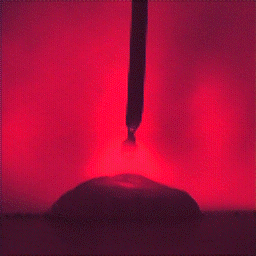
\includegraphics[width=3.5cm,height=3.5cm]{images/photo-macro-drop-original.png}}
\subfigure[Macro drop grayness image]{\label{photo-macro-drop-grey}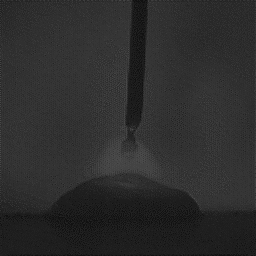
\includegraphics[width=3.5cm,height=3.5cm]{images/photo-macro-drop-grey.png}}\\
\subfigure[First smooth filter]{\label{photo-macro-drop-smoothblur}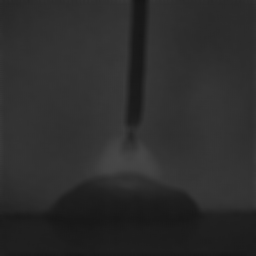
\includegraphics[width=3.5cm,height=3.5cm]{images/photo-macro-drop-smoothblur.png}}
\subfigure[Adaptive threshold per regions]{\label{photo-macro-drop-adaptivethreshold}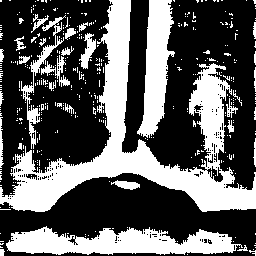
\includegraphics[width=3.5cm,height=3.5cm]{images/photo-macro-drop-adaptivethreshold.png}}\\
\subfigure[Median filter]{\label{photo-macro-drop-smoothmedian}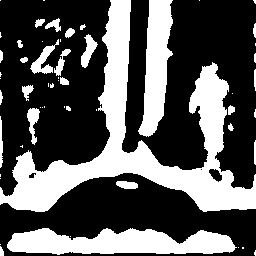
\includegraphics[width=3.5cm,height=3.5cm]{images/photo-macro-drop-smoothmedian.png}}
\subfigure[Canny filter]{\label{photo-macro-drop-canny}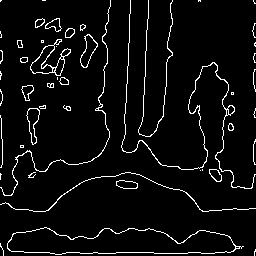
\includegraphics[width=3.5cm,height=3.5cm]{images/photo-macro-drop-canny.png}}\\
\end{center}
\caption{{\small Image treatment step by step of PGMAW process}}
\label{photo-macro-drop}
\end{figure}


\subsection{Edge extraction}
\label{edge_extraction}
Despite performance achieve by the image treatment, Canny filter
 generate many edges, or cords, in the image. These cord are composed
 by white pixels, interpreted by the algorithms as an individuals points.
 In order to automate the edge extraction process, geometrical and
 graph algorithms are used  to isolate the cords corresponding to
 macro drop profile and edge section droplet.

To the macro drop profile a user interaction algorithm is responsible
 to extract the continuous cord (white pixels) corresponding
 to the profile into a list. Note  that the macro drop and 
the substrate have the same continuous profile (see figure \ref{photo-macro-drop-canny}.
 The substrate shadow projection is always the same if the optical
 path doesn�t change. Therefore the users have only to choose, to
 first image in the experience series, one extreme  of the cord 
corresponding to substrate profile (see figures \ref{photo-results-macro-drop}).
 Then the algorithm finds all new white pixels inside small neighbor around
 the pixels selected by the user. Each new white pixel  is added to the
 profile list. Starting at each new pixel, this process continues,
 automatically, until the other extreme of the cord, until the last
 image of the series.
 
\begin{figure}[h!]
\begin{center}    
\subfigure[t = ]{\label{photo-results-macro-drop-t1}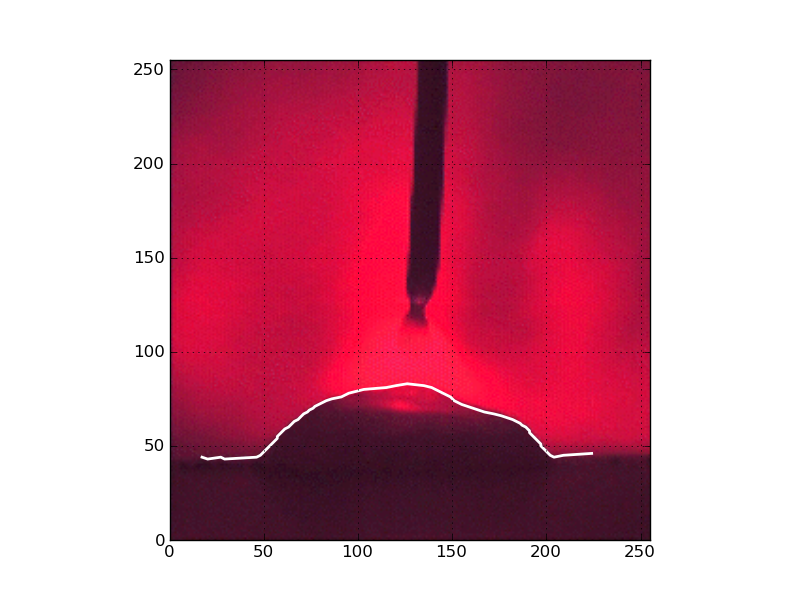
\includegraphics[width=3.5cm,height=3.5cm]{images/photo-results-macro-drop-t1.png}}
\subfigure[t = ]{\label{photo-results-macro-drop-t2}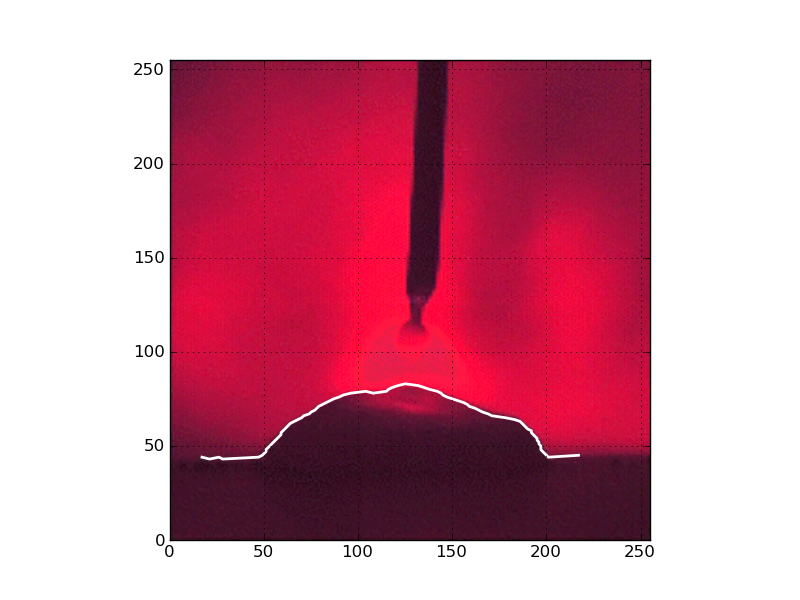
\includegraphics[width=3.5cm,height=3.5cm]{images/photo-results-macro-drop-t2.png}}\\
\subfigure[t = ]{\label{photo-results-macro-drop-t3}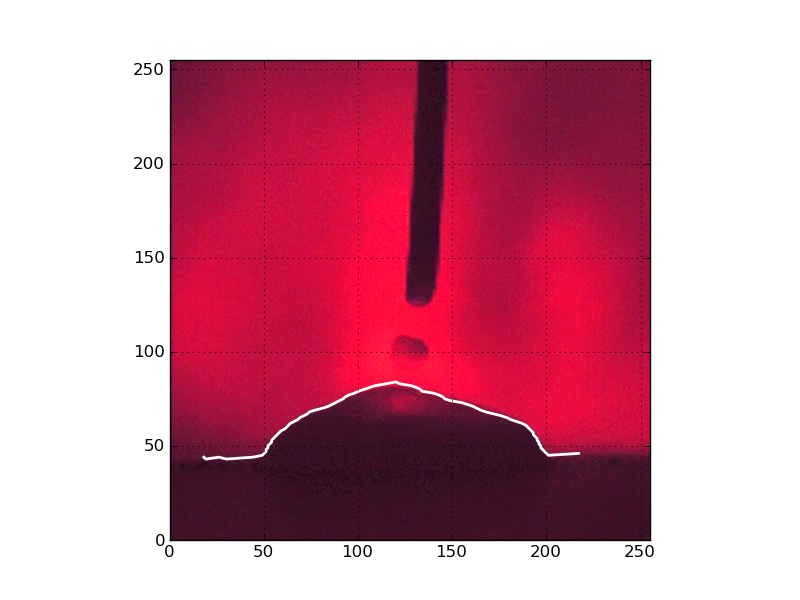
\includegraphics[width=3.5cm,height=3.5cm]{images/photo-results-macro-drop-t3.png}}
\subfigure[t = ]{\label{photo-results-macro-drop-t4}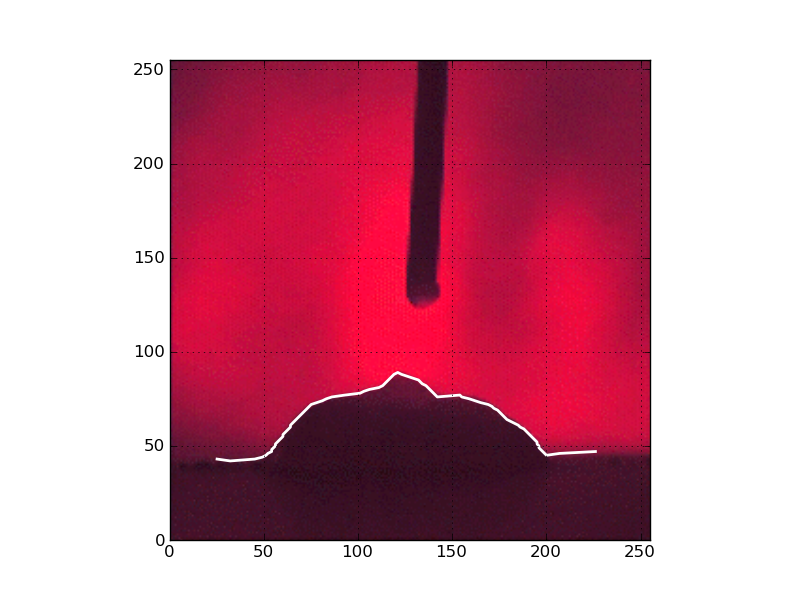
\includegraphics[width=3.5cm,height=3.5cm]{images/photo-results-macro-drop-t4.png}}\\
\end{center}
\caption{{\small Images series of macro drop profiles}}
\label{photo-results-macro-drop}
\end{figure}
               
               
To the droplet edge section, the white points cord defines 
the surface of the droplet. Note at figure \ref{photo-droplet-canny} that the biggest closer
 cord correspond to the droplet section. The idea is to build segments around
 the cords, and take the longest closer segment. 
                
                
Give $S$ the set of points in the space image. The segments could 
be building between wherever two points of $S$. However, to fulfill
 the cords with segments, only the points placed together could define
 a segment. To choose the correct points of $S$ a Delaunay triangulation
 is made over $S$ \cite{CGAL}. Each point of $S$ is a vertices 
of a triangle and then each potential segment is a side of a triangle. 
The Delaunay triangulations guarantee a unique solution with minimal internal angles for each triangle, which means  minimal length sides to the triangles \cite{GEOMETRICAL}.
 Give $\beta$ the cord surrounding the external hull of the Delaunay
 triangulation of $S$. An alpha shape algorithm uses a $\alpha \in N$ parameter,
 or square radius of a test circle, to travel from outside $\beta$ to inside
 the triangulation. The circle has to go through the triangles sides without touch the vertices. Give 
$n$ the number of triangles sides of triangulation
and $l_{i}$ with $i\in\{1,n\}$ the length of each side, if $\sqrt{\alpha} > l_{i}$ 
with $i \in\{1,n\}$, a segment is build between the respective vertices or
 points. At the end of the process, a segments set know as $\alpha$-shape has been created.  Note if $\sqrt{\alpha} > l_{i} \forall i$, the circle can�t be go inside $\beta$, then $\alpha$-shape
 is $\beta$ \cite{CGAL}. If $\sqrt{\alpha} < l_{i} \forall i$ the circle go through
 every side in the triangulation,  then no segment are created and $\alpha$-shape
 became $S$. The points that compound the droplet section are all contact neighbors. Then $\alpha = 1$
 is sufficient to create a segment set around the droplet
 (see figure \ref{photo-droplet-alpha-shape}). 
                                  
\begin{figure}[h!]
\begin{center}    
\subfigure[t = ]{\label{photo-droplet-canny}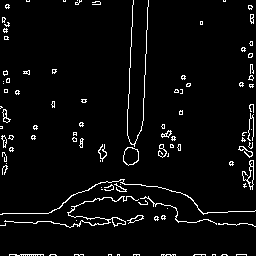
\includegraphics[width=3.5cm,height=3.5cm]{photo-droplet-canny.png}}
\subfigure[t = ]{\label{photo-droplet-alpha-shape}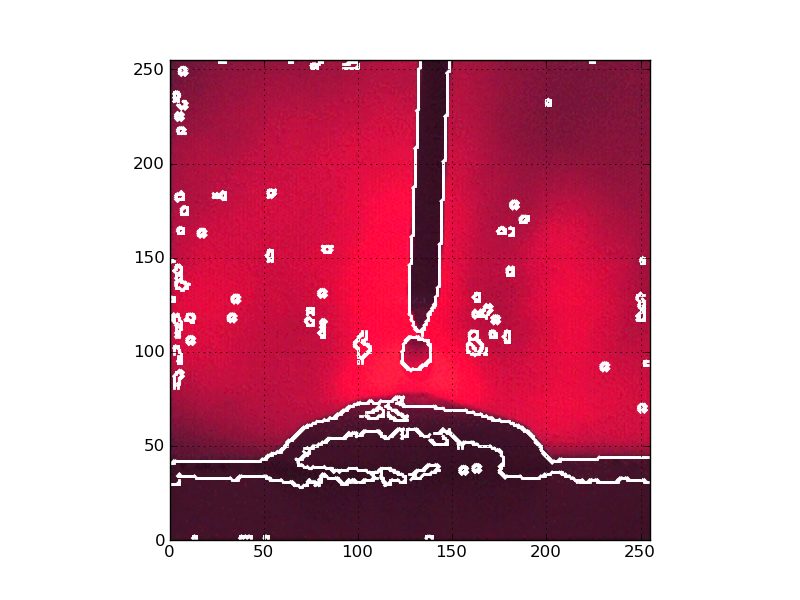
\includegraphics[width=3.5cm,height=3.5cm]{photo-droplet-alpha-shape.png}}\\
\end{center}
\caption{{\small Images series of macro drop profiles}}
\label{photo-results-droplet}
\end{figure}

A graph algorithm connects this segment and finds the longest closer segment. The longest closer segment corresponds to the metal transfer drop profile 
(see figure \ref{photo-results-droplet}).

\begin{figure}[h!]
\begin{center}    
\subfigure[t = ]{\label{photo-results-droplet-t1}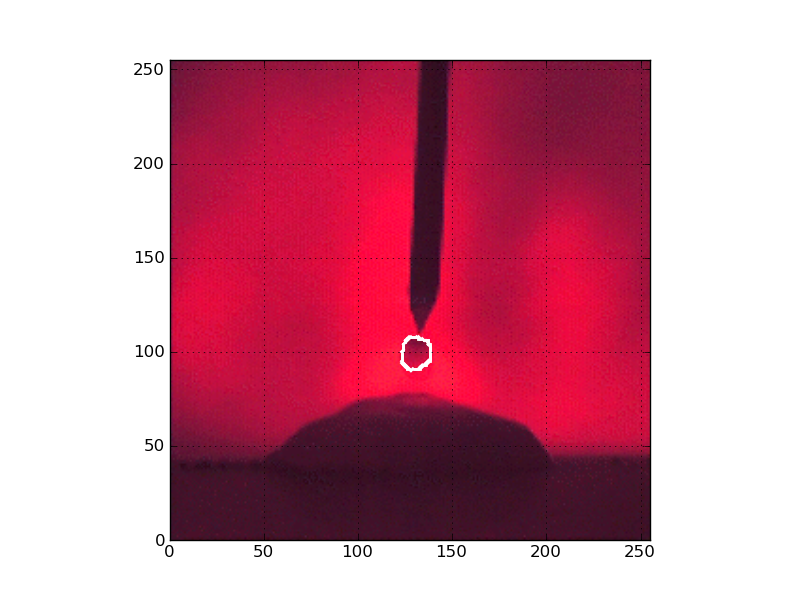
\includegraphics[width=3.5cm,height=3.5cm]{images/photo-results-droplet-t1.png}}
\subfigure[t = ]{\label{photo-results-droplet-t2}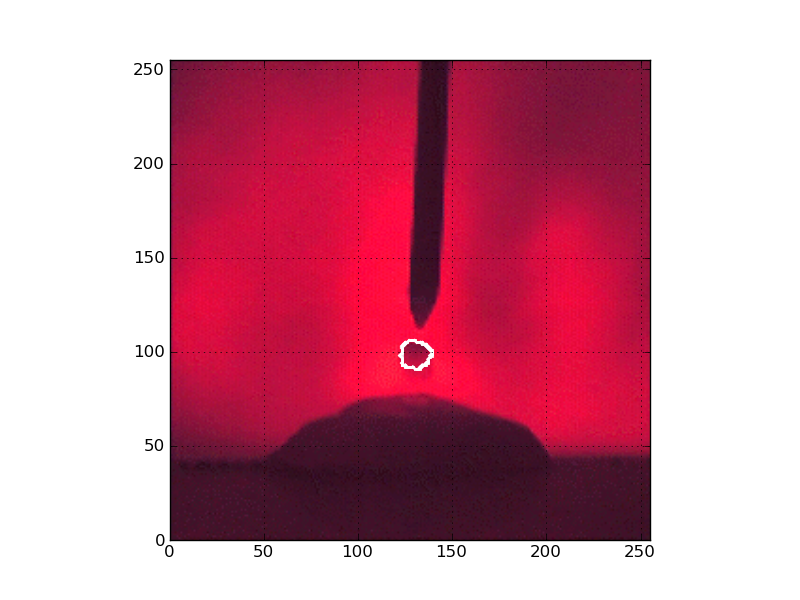
\includegraphics[width=3.5cm,height=3.5cm]{images/photo-results-droplet-t2.png}}\\
\subfigure[t = ]{\label{photo-results-droplet-t3}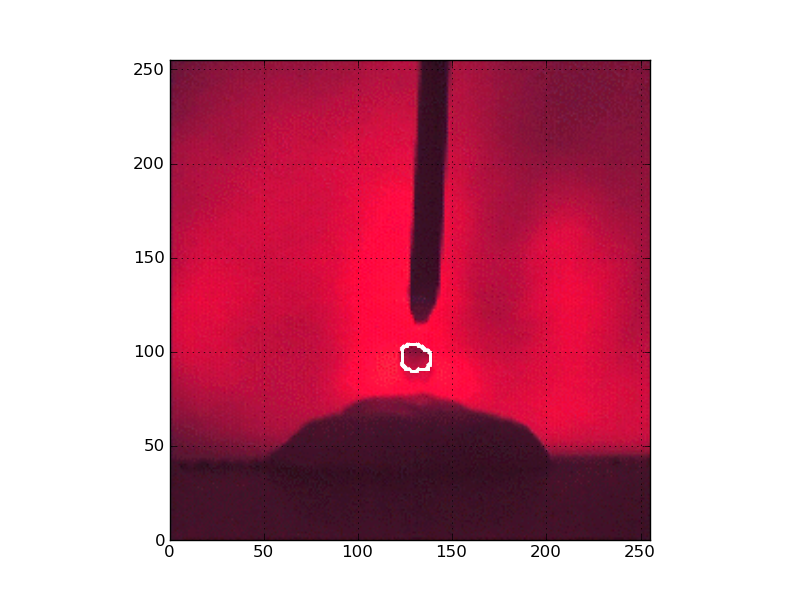
\includegraphics[width=3.5cm,height=3.5cm]{images/photo-results-droplet-t3.png}}
\subfigure[t = ]{\label{photo-results-droplet-t4}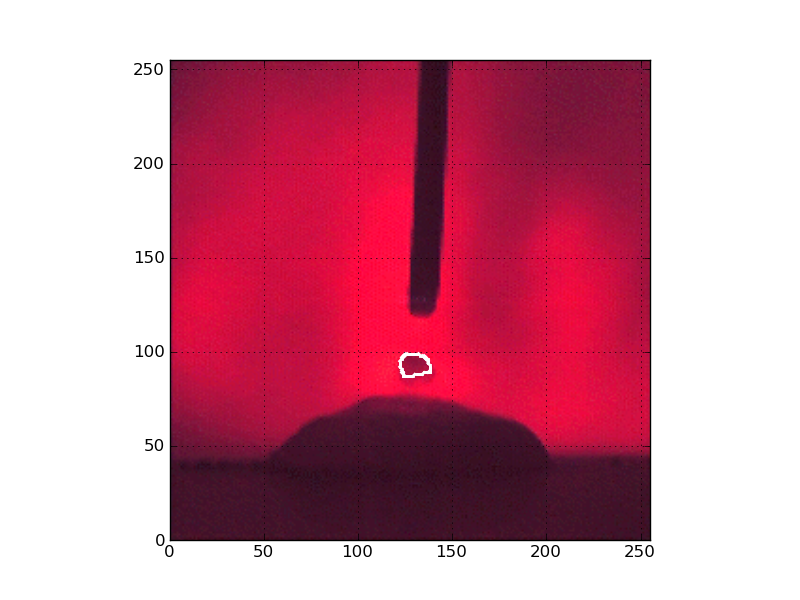
\includegraphics[width=3.5cm,height=3.5cm]{images/photo-results-droplet-t4.png}}\\
\end{center}
\caption{{\small Images series of macro drop profiles}}
\label{photo-results-droplet}
\end{figure}


\subsection{Geometrical Analysis}
\label{geometrical_analize}

Now it is possible to determine the geometrical parameters shown 
at figure \ref{schema-macro-drop-droplet-parameters}. To compute the wetting 
angle measures, linear regressions or least squares (parabolic, ellipse, circle) 
are taken from the processed macro drop extracted profiles.
A loop algorithm applies this method to all frames at the experience to compute the wetting 
angles. Same procedure is use to estimate the macro drop radius and volume \cite{CHAPUIS}.



\section{ Results}
In this part some results, performance and reliability of the library for a set of experiment
are shown. The basic experiment is static Pulse Gas Tungsten Arc Welding.
A macrodrop is feed by droplets at a frequency of 110 Hertz. The droplets are assumed to flight vertically and
then to feed the macro drop generated. The macrodrop grows with a geometry that depends on the effects of gravity
but also of surface tension,.....
For the same welding parameters, the shielding gas will be modified and the modification of
the advance of the basis radius will be demonstrated. 

To improve weld quality in pulsed GMAW, the dynamic of the droplet is investigated.
The analysis focus on the regularity of the transfert and some statistics are shown.

Some analysing time are given in order to appreciate the performance of the library with sophisticated
algorithm.


\subsection{ Macro Drop growth investigation}
The investigation of the macro drop growth needs the study of two quantities:

\begin{itemize}
\item The angle between the substrate and the liquid
\item The speed of growth of the macro drop radius
\end{itemize}

The macro drop is assumed to be axisymmetric so this two quantities are representative of the 
geometry or its evolution.

\subsection{ Droplet flight}


\section{ Conclusions}

\bibliography{paper_bain}

%\section*{References}
%\begin{thebibliography}{10}
%\bibitem{book1} Goosens M, Rahtz S and Mittelbach F 1997 {\it The \LaTeX\ Graphics Companion\/} 
%(Reading, MA: Addison-Wesley)
%\bibitem{eps} Reckdahl K 1997 {\it Using Imported Graphics in \LaTeX\ } (search CTAN for the file `epslatex.pdf')
%\end{thebibliography}
\bibitem{CGAL} http://www.cgal.org 
\end{document}

